% OWNER: Maryam Fatima
\section{CAVR: Dependency and Package Trust}\label{sec:cavr}
\begin{sloppypar}
CAVR stands between a dependency request and the project environment. In this iteration I built its fast gate: one function, \path{verify_request} in \path{backend/cavr/pipeline.py}, that takes a \texttt{pip install} command or a \path{requirements.txt} edit and returns \texttt{VERIFIED}, \texttt{REJECTED}, \texttt{UNRESOLVED} or \texttt{BLOCK} with the evidence for each stage. The pip wrapper and the CAVR page of the dashboard both call this one function. The work is on branch \href{https://github.com/SheharyarAli-Dev/Working-POC/tree/cavr}{\texttt{cavr}}, head commit \texttt{d63183d}.
\end{sloppypar}

\subsection{Design}
\begin{sloppypar}
The mid goals were written down before the work started as C1 to C4: C1 capture a real \texttt{pip install X==Y} or a \path{requirements.txt} edit; C2 a requirement gate that blocks at once when the policy does not permit the request; C3 a fast gate on real PyPI artifacts (SHA-256 of the downloaded file against the registry digest, the transitive tree from real \texttt{Requires-Dist} metadata, OSV with version-range checks, a light AST scan, and a verdict cache); C4 a capability contract taken from the project's real imports and call sites. Two rules applied to every goal: no result comes from fixture data, and anything unknown is \texttt{UNRESOLVED}. C1 to C4 are the first four phases of the CAVR flow in the integrated ASENT design, which numbers the flow C1 to C12. That design also sets the eight fields of the cache key and names cache hit rate and p50/p95 latency as metrics to report.
\end{sloppypar}

The pipeline runs nine stages in a fixed order. Each stage adds its result to the evidence of the verdict.

\setlength{\tabcolsep}{3pt}
\begin{longtable}{p{0.04\textwidth}p{0.17\textwidth}p{0.25\textwidth}p{0.45\textwidth}}
\toprule
\textbf{No.} & \textbf{Stage} & \textbf{Module} & \textbf{What it produces and when it stops the request}\\
\midrule
\endhead
1 & C1 capture & \path{capture.py}, \path{manifest_parser.py} & The request as a structured record. Unsupported or unreadable input marks the record incomplete.\\
2 & C2 requirement gate & \path{requirement_gate.py} & \texttt{PERMITTED}, \texttt{BLOCK} or \texttt{UNRESOLVED} from the policy, allowlist and lockfile. \texttt{BLOCK} stops here, before any download.\\
3 & C3 artifact & \path{pypi_client.py} & The real wheel in a quarantine directory, with the SHA-256 of the bytes on disk and the registry digest. A mismatch is \texttt{REJECTED}.\\
4 & C3 tree & \path{dep_tree.py}, \path{wheel_meta.py} & Every dependency from real \texttt{Requires-Dist} lines, each downloaded and hashed, and one subtree digest.\\
5 & C4 contract & \path{context_extractor.py}, \path{capability_contract.py} & The project's imports and call sites of the package, and the allowed and denied capabilities.\\
6 & Cache lookup & \path{verdict_cache.py} & \texttt{HIT} or \texttt{MISS} on the eight-field key. The key needs the results of stages 3, 4 and 5.\\
7 & Advisories & \path{advisories.py} & The OSV answer for every package of the tree, on every run. An affected version is \texttt{REJECTED}.\\
8 & AST scan & \path{ast_scan.py}, \path{reachability.py} & On a cache miss only: the sinks found in the wheel sources, each judged against the contract and against reachability from the project.\\
9 & Verdict & \path{pipeline.py} & \texttt{VERIFIED}, \texttt{REJECTED} or \texttt{UNRESOLVED}, or \texttt{BLOCK} from stage 2.\\
\bottomrule
\end{longtable}
\setlength{\tabcolsep}{6pt}

The verdict follows four rules, taken from the module's own header:
\begin{sloppypar}
\begin{itemize}
    \item \texttt{REJECTED} when the downloaded bytes do not match the registry, a wheel is unsafe, or OSV lists the version of the package or of anything in its tree as affected.
    \item \texttt{UNRESOLVED} when anything is unknown: the request, the policy, the network, a dependency that is not pinned, a project that cannot be read, a package the project never uses, or code the scan cannot read.
    \item A sensitive sink in a wheel is evidence, not a failure, unless the contract does not allow its capability outright and the project's call sites can reach it. Then the verdict is \texttt{UNRESOLVED} and carries the escalation text ``deep analysis required (M2)''.
    \item With several requirements in one request: \texttt{REJECTED} if any is rejected, else \texttt{UNRESOLVED} if any is unresolved, else \texttt{VERIFIED}.
\end{itemize}
\end{sloppypar}
No stage installs, imports or runs package code.

\textbf{Interfaces.} CAVR has three entry points and all three reach the same function.
\begin{sloppypar}
\begin{itemize}
    \item \textbf{Python:} \path{verify_request(request,project_dir,policy,store)}. The request is a pip command, a requirements edit or a capture record. The result is a dictionary with \texttt{status}, \texttt{stage}, \texttt{rule}, \texttt{reason}, \texttt{fast\_gate\_ms}, \texttt{cache\_hit}, \texttt{escalated}, \texttt{gate}, \texttt{packages} and \texttt{policy\_version}.
    \item \textbf{Command line:} \texttt{python} \path{-m} \path{backend.cavr.pip_shim} \texttt{install} \path{<name>==<version>}, with the wrapper options \path{--cavr-project}, \path{--cavr-policy}, \path{--cavr-python}, \path{--cavr-json} and \path{--install}. Exit code 0 is \texttt{VERIFIED}, 1 \texttt{REJECTED}, 2 \texttt{UNRESOLVED}, 3 \texttt{BLOCK}, and 4 means an install was asked for after a \texttt{VERIFIED} verdict and pip did not succeed.
    \item \textbf{HTTP:} \texttt{GET} \path{/api/cavr/scenarios} lists the six request chips; \texttt{POST} \path{/api/cavr/run?scenario=<id>} and \texttt{POST} \path{/api/cavr/intercept} start a run; \texttt{GET} \path{/api/cavr/stream/{run_id}} replays the run's events; \texttt{GET} \path{/api/cavr/proof/{run_id}} returns the verdict, the hash comparison and the six-stage summary; \texttt{GET} \path{/api/cavr/metrics} and \texttt{GET} \path{/api/cavr/cache} return the report numbers and the stored cache rows.
\end{itemize}
\end{sloppypar}

\begin{sloppypar}
\textbf{Data.} The policy is one JSON file with \texttt{approved\_requirements}, \texttt{denied\_packages}, \texttt{allowed\_scopes} and \texttt{project\_task\_description}. Its version is the SHA-256 of its canonical JSON. SQLite holds two CAVR tables in \path{backend/cavr/storage.py}: \texttt{verdict\_cache}, one row per cache key with the eight key fields as columns and an integrity digest, and \texttt{verdict\_log}, one row per \path{verify_request} call. Downloaded wheels go to \path{cavr/quarantine} under the data directory named by \texttt{ASENT\_DATA}.
\end{sloppypar}

\begin{sloppypar}
\textbf{Change from the proposal design.} The CAVR design document describes the same flow in more detail as thirteen phases, P1 to P13. This iteration implements P1 capture, P2 requirement gate, P3 context, P4 capability contract and P5 package resolution, and the static part of P6: the AST scan lists sinks and environment-gated triggers but does not rank them. P7 to P12 (counterfactual sandbox, OS observation, causal verification, repair, re-verification and reconstruction) are not part of the fast gate. Three further differences from the design document are deliberate for this stage. The design lists PyPI and npm; the fast gate handles PyPI wheels only. The design lists four outcomes including \texttt{RESTRICTED}; the fast gate returns \texttt{VERIFIED}, \texttt{REJECTED} and \texttt{UNRESOLVED}, plus \texttt{BLOCK} from the gate, and has no \texttt{RESTRICTED}. The design's context phase reads the Git diff; the implemented context extractor reads the project's Python files with \texttt{ast} and no longer runs \texttt{git diff}, because nothing used its output.
\end{sloppypar}

\begin{sloppypar}
\textbf{Change from the proposal prototype.} Before this iteration the CAVR dashboard showed results from fixture scenarios in \path{backend/cavr/fixtures/scenarios.py}, and parts of it wrote fixed text. The old certificate function wrote ``MET 98\%'' and ``honeytoken CLEAN'' from the verdict word alone, and the sandbox runner returned a made-up report when Docker was missing. All of that is removed from the path the dashboard uses. \path{backend/cavr/api.py} no longer imports the fixture, resolver, re-verifier, reconstructor, trigger, counterfactual, normalizer, causal-graph or repair-engine modules. Those files are still in the repository and are not used by the app's CAVR page.
\end{sloppypar}

\subsection{Implementation}
The files below were added or rewritten in this iteration. All are in \path{backend/cavr/}. Line counts are at commit \texttt{d63183d}.

\setlength{\tabcolsep}{3pt}
\begin{longtable}{p{0.27\textwidth}p{0.07\textwidth}p{0.57\textwidth}}
\toprule
\textbf{File} & \textbf{Lines} & \textbf{Classes, functions and what they do}\\
\midrule
\endhead
\path{capture.py} & 460 & \path{parse_pip_command}, \path{parse_requirement}, \path{parse_requirements_text}, \path{redact}. Turns a pip command into a capture record using explicit option tables.\\
\path{manifest_parser.py} & 170 & \path{snapshot_requirements}, \path{capture_requirements_edit}. Compares two snapshots of a requirements file and records added, changed and removed lines.\\
\path{requirement_gate.py} & 319 & \path{evaluate_requirement}, \path{evaluate_capture}, \path{gate_from_files}, \path{policy_version}; class \path{Unreadable} for a policy or lockfile that exists and is not usable JSON. The fail-closed requirement gate.\\
\path{pypi_client.py} & 303 & \path{fetch_artifact}, \path{select_wheel}; classes \path{HttpxTransport} (HTTPS, no redirects) and \path{TransportError} (the one exception a transport raises). Reads the PyPI release JSON, downloads one wheel into quarantine and checks its SHA-256.\\
\path{wheel_meta.py} & 268 & \path{read_wheel}, \path{check_entries}; exception class \path{WheelProblem}. Checks the zip budget and paths, then reads \texttt{METADATA}, \texttt{WHEEL} and the import names.\\
\path{dep_tree.py} & 258 & \path{build_tree}, \path{subtree_digest}. Builds the transitive tree from \texttt{Requires-Dist} and the lockfile.\\
\path{advisories.py} & 200 & \path{check_advisories}, \path{match_advisory}, \path{summarise_ids}. Asks OSV and evaluates each advisory's ranges for the version.\\
\path{ast_scan.py} & 260 & \path{scan_wheel}. Parses every Python file of a wheel and reports sinks, triggers, dynamic code and what it could not read.\\
\path{context_extractor.py} & 273 & \path{extract_project_context}, \path{usage_of}; class \path{_Uses}, an \path{ast.NodeVisitor} that maps each local name to its real dotted name. Reads the project's Python files and records imports, call sites and references.\\
\path{capability_contract.py} & 347 & \path{infer_capability_contract}, \path{vocabulary}, \path{use_through_local_artifacts}. Builds the contract and its digest.\\
\path{reachability.py} & 409 & \path{judge_sinks}, \path{import_graph}; class \path{ProjectSources}. Gives each sink one of \texttt{ALLOWED}, \texttt{GUARD\_DISABLED}, \texttt{UNREACHABLE}, \texttt{REACHABLE}.\\
\path{verdict_cache.py} & 149 & \path{cache_key}, \path{lookup}, \path{store}, \path{row_integrity}. The eight-field verdict cache.\\
\path{pipeline.py} & 436 & \path{verify_request}, \path{metrics}, \path{analyzer_version}. Runs the nine stages and writes the verdict log.\\
\path{pip_shim.py} & 287 & \path{main}, \path{split_arguments}, \path{install_plan}, \path{render}. The pip wrapper.\\
\path{api.py} & 589 & \path{run_verification}, \path{verdict_events}, \path{stage_summary}, \path{SCENARIOS}; classes \path{TamperingTransport} and \path{OfflineTransport} for the two demo conditions. The dashboard endpoints.\\
\path{assurance.py} & 251 & \path{certificate_for_verdict}; class \path{EvidenceChain}, the hash chain of run events. A certificate that copies the verdict and adds nothing of its own.\\
\path{storage.py} & 326 & Class \path{CavrStorage}: tables \texttt{verdict\_cache} and \texttt{verdict\_log} with their read and write methods.\\
\path{sandbox_runner.py} & 188 & Class \path{SandboxRunner}, method \path{run}. Host fallback removed; no Docker or no usable report gives \texttt{UNRESOLVED}.\\
\bottomrule
\end{longtable}
\setlength{\tabcolsep}{6pt}

\begin{sloppypar}
The page itself is \path{frontend/src/components/CavrModule.tsx} with the components in \path{frontend/src/components/cavr/}: \path{ScenarioChips.tsx}, \path{Timeline.tsx}, \path{ProofDrawer.tsx}, \path{AdvisoryList.tsx} and \path{MetricsTab.tsx}. The page holds no package name and no result string of its own. It reads the chips from \texttt{GET} \path{/api/cavr/scenarios} and prints a dash for any value the API did not compute.
\end{sloppypar}

\begin{sloppypar}
The policy used by the dashboard and the demo is \path{backend/cavr/project_policy.json}. It approves \texttt{pypdf>=5,<7}, grants \texttt{FILE\_READ:invoice\_documents} and \texttt{FILE\_WRITE:scratch\_tmp}, and sets \texttt{PROCESS\_EXEC:none} and \texttt{NETWORK\_CONNECT:none}. The protected project is \path{backend/cavr/sample_project}, an invoice reader that uses pypdf.
\end{sloppypar}

\subsection{Completed Features}
\begin{itemize}
    \item Capture of \texttt{pip install} commands and of \path{requirements.txt} edits into one record format.
    \item A requirement gate with denylist, pin, allowlist and lockfile rules that blocks before any download.
    \item Download of the real wheel from PyPI with a SHA-256 check of the file on disk against the registry digest.
    \item Safe reading of wheel metadata with a zip budget and path checks.
    \item A transitive dependency tree from real metadata, with a subtree digest.
    \item An OSV advisory check that evaluates version ranges, for every node of the tree, on every run.
    \item An AST scan of wheel sources that reports sinks, triggers and what it could not read.
    \item A capability contract from the project's own imports and call sites, and a sink judgement against it.
    \item A verdict cache on an eight-field key with tamper detection.
    \item A pip wrapper with exit codes and an optional hash-pinned install.
    \item A dashboard page with six real request chips, a six-stage timeline, a proof drawer, an advisory list and a metrics tab.
    \item A sandbox runner that never runs package code on the host.
\end{itemize}
Not completed in this iteration: sandbox execution of packages, counterfactual activation, the causal graph, repair and re-verification. The tabs for them on the CAVR page say ``Not run''.

\subsection{Technical Implementation Details}
\begin{sloppypar}
\textbf{Capture.} \path{parse_pip_command} splits the command with \texttt{shlex}, finds the tokens after \texttt{pip} or \texttt{python -m pip}, and separates options from positionals using three option tables. Only the \texttt{install} subcommand is captured. A positional goes to \path{parse_requirement}, which classifies it as a named requirement, an unsupported form (VCS, URL, local path) or an error. A \texttt{-r} or \texttt{-c} file is read only if it is inside the directory the command ran in, is at most 1\,000\,000 bytes and is valid UTF-8. Nested includes are followed with a stack, so a file that includes itself ends as an error. The record is complete only when it has no unsupported entry and no error.
\end{sloppypar}

\begin{sloppypar}
\textbf{Requirement gate.} \path{evaluate_requirement} applies the first rule that fits: no policy gives \texttt{UNRESOLVED} \texttt{POLICY\_MISSING}; an unusable policy gives \texttt{POLICY\_INVALID}; a name on the denylist gives \texttt{BLOCK} \texttt{DENYLIST}; anything but exactly one \texttt{==} clause gives \texttt{BLOCK} \texttt{NOT\_PINNED}; no allowlist entry whose specifier contains the version gives \texttt{BLOCK} \texttt{NOT\_ON\_ALLOWLIST}; with a lockfile, no entry with the same name and version gives \texttt{BLOCK} \texttt{NOT\_IN\_LOCKFILE}. Only after all of these does it return \texttt{PERMITTED} \texttt{ALLOWED}. The gate parses the request again and recomputes completeness itself; it does not trust the flags of the record it is given.
\end{sloppypar}

\begin{sloppypar}
\textbf{Artifact.} \path{fetch_artifact} reads \path{https://pypi.org/pypi/{name}/{version}/json}, picks the wheel the running interpreter would install (\path{packaging.tags.sys_tags()}), and checks the chosen entry before downloading: not yanked, hosted on \path{files.pythonhosted.org} over HTTPS, a 64-hex \texttt{sha256} present. It streams the file to a \texttt{.part} file in quarantine, opens that file again, hashes it, and renames it to its wheel name on a match or to \path{<filename>.rejected} on a mismatch. Redirects are not followed.
\end{sloppypar}

\begin{sloppypar}
\textbf{Wheel metadata and tree.} \path{read_wheel} checks the zip directory before reading any entry: entry count, declared uncompressed size, compression ratio, absolute paths, \texttt{..} parts, symlinks and duplicate names. It then requires exactly one \texttt{dist-info} directory and compares the name and version in \texttt{METADATA} with the directory name and with the request. \path{build_tree} starts from the requested package, loads each node once, evaluates the marker of every \texttt{Requires-Dist} line for the running interpreter, and pins each child from the lockfile. A child with no single matching lockfile version makes the tree \texttt{UNRESOLVED}. The subtree digest is the SHA-256 of the sorted nodes (name, version, SHA-256) and sorted edges.
\end{sloppypar}

\begin{sloppypar}
\textbf{Advisories.} \path{check_advisories} queries OSV for the canonical name and version and passes every returned advisory to \path{match_advisory}, which walks the events of each ecosystem range (\texttt{introduced} inclusive, \texttt{fixed} exclusive, \texttt{last\_affected} inclusive). Any affected advisory gives \texttt{REJECTED} \texttt{KNOWN\_VULNERABILITY}. A range that cannot be evaluated gives \texttt{UNRESOLVED} \texttt{RANGE\_UNSUPPORTED}. If OSV returned an advisory and the local range check says the version is not affected, the two disagree and the result is \texttt{UNRESOLVED} \texttt{RANGE\_DISAGREEMENT}. PyPI's own advisory list is not accepted as an answer, because it has no ranges to check.
\end{sloppypar}

\begin{sloppypar}
\textbf{AST scan.} \path{scan_wheel} parses every \texttt{.py} and \texttt{.pyw} entry with \texttt{ast} and runs the threat-repository sink and trigger rules on it. A second pass maps import aliases such as \texttt{from subprocess import run} to full names, so a sink called through an alias is still found. Lines of a \texttt{.pth} file that start with \texttt{import} are code that Python runs at start-up; they are scanned and make the result \texttt{UNRESOLVED}. Native files, bytecode-only files and files that do not parse also make it \texttt{UNRESOLVED}. Finding a sink does not change the scan result; the sink is judged in the next step.
\end{sloppypar}

\begin{sloppypar}
\textbf{Capability contract and sink judgement.} \path{extract_project_context} walks the project without following links and records, per file, each import and each use of an imported name as a call, a decorator or a reference. \path{infer_capability_contract} takes the import names from the wheel metadata, never from the distribution name, selects the project's uses of those names, and combines the policy's \texttt{allowed\_scopes} with the threat-repository capability rules into allowed and denied capabilities. A package the project imports nowhere, or imports and never uses, has no call-site authority and is \texttt{UNRESOLVED}. \path{judge_sinks} then builds the import graph over all wheels of the tree and takes the closure from the modules the project imports. A sink whose capability is granted with scope \texttt{*} is \texttt{ALLOWED}; a sink outside the closure is \texttt{UNREACHABLE}; any other sink is \texttt{REACHABLE} and makes the verdict \texttt{UNRESOLVED}.
\end{sloppypar}

\begin{sloppypar}
The demo package shows why the last step is needed. pypdf 6.19.0 calls \texttt{subprocess.run} at \path{pypdf/filters.py:774} and \path{pypdf/filters.py:804} for its optional JBIG2 decoder, and the policy sets \texttt{PROCESS\_EXEC:none}. The sample project creates and uses every \texttt{PdfReader} inside \path{apply_configuration(jbig2dec_binary=None)}, which switches that decoder off. \path{judge_sinks} accepts this as a \texttt{GUARD\_DISABLED} proof only under strict conditions: pypdf is the requested package, \texttt{PdfReader} and \texttt{apply\_configuration} are imported only as \texttt{from pypdf import ...}, and every reader is created and used inside the guard block. The same project with a reader outside the guard is \texttt{UNRESOLVED} and escalated. This proof is written for pypdf only.
\end{sloppypar}

\begin{sloppypar}
The CAVR page prints this contract and this judgement for the demo request, as shown in Figure~\ref{fig:cavr-capability-contract}: four call sites, \texttt{FILE\_READ} and \texttt{FILE\_WRITE} required and permitted, the other eight capabilities denied, and the two \texttt{subprocess.run} sinks listed against \texttt{PROCESS\_EXEC} with the result ``No reachable sink''. Figure~\ref{fig:cavr-ast-scan} shows the scan behind that row: 59 Python files read, both sinks judged \texttt{GUARD\_DISABLED} by the accepted proof \texttt{pypdf-jbig2dec-disabled}, and the limit of that proof as the page states it. Both are static findings; no package code was run.
\end{sloppypar}

\begin{figure}[htbp]
    \centering
    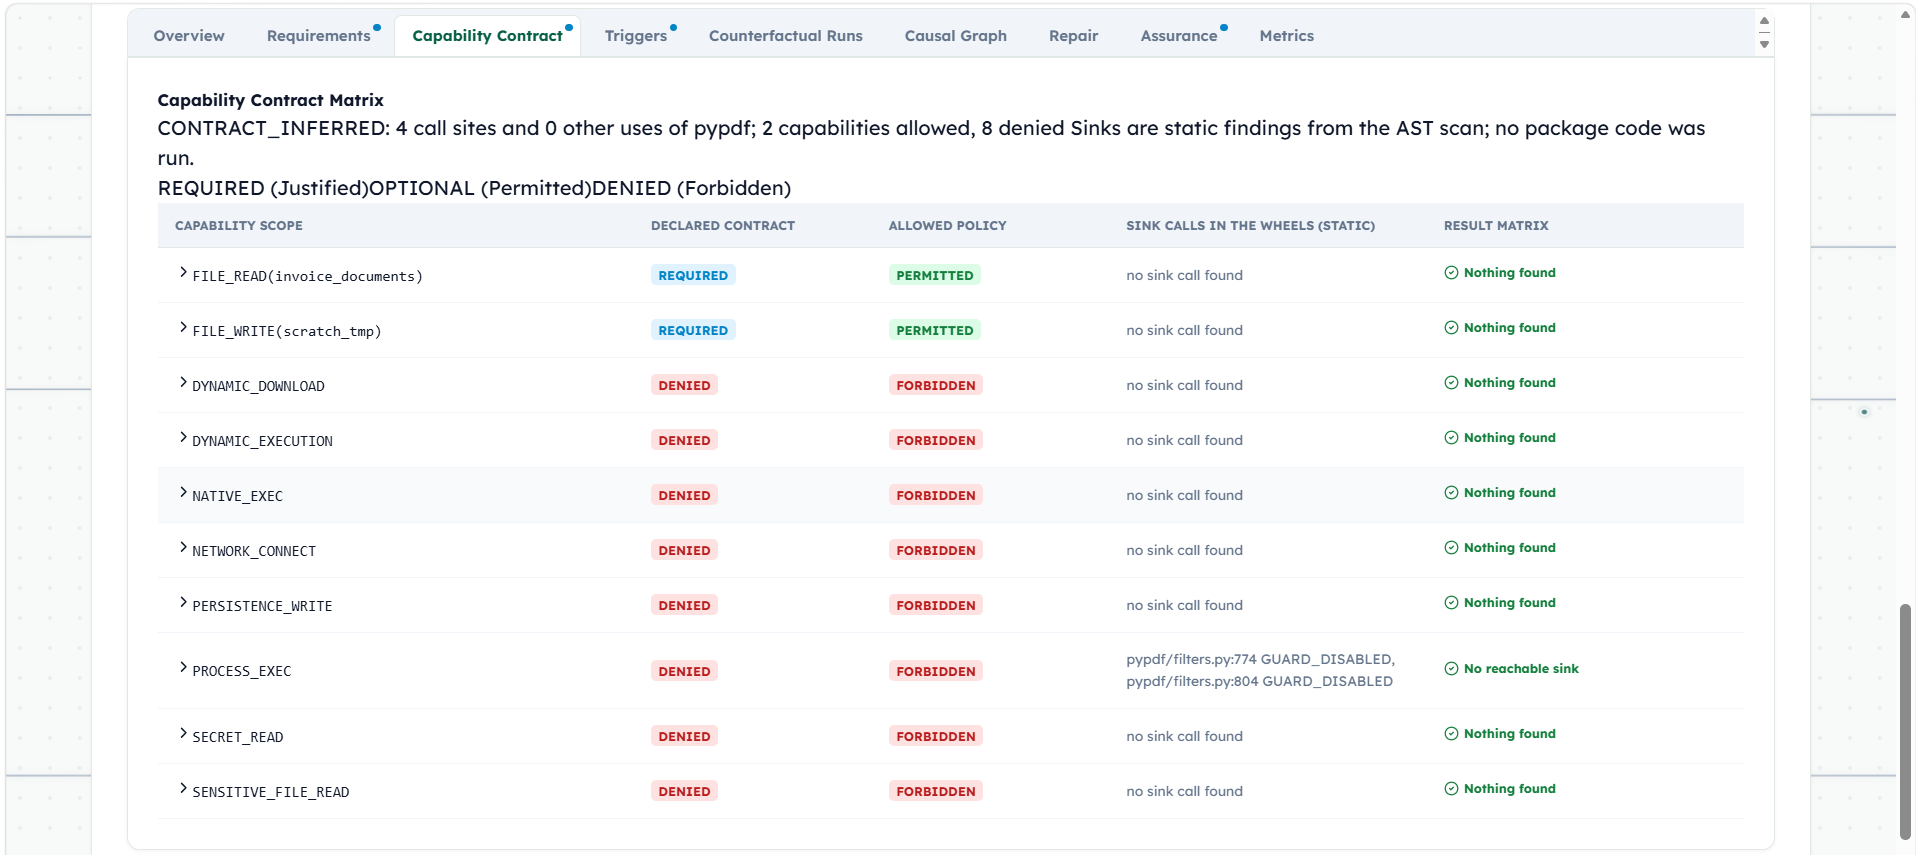
\includegraphics[width=0.9\linewidth]{figures/cavr/cavr-11-capability-contract.png}
    \caption[Capability contract inferred for pypdf 6.19.0]{Capability contract tab for \texttt{pypdf} 6.19.0 in the sample project: two capabilities required and permitted, eight denied, and the two \texttt{subprocess.run} sinks under \texttt{PROCESS\_EXEC} judged \texttt{GUARD\_DISABLED}.}
    \label{fig:cavr-capability-contract}
\end{figure}

\begin{figure}[htbp]
    \centering
    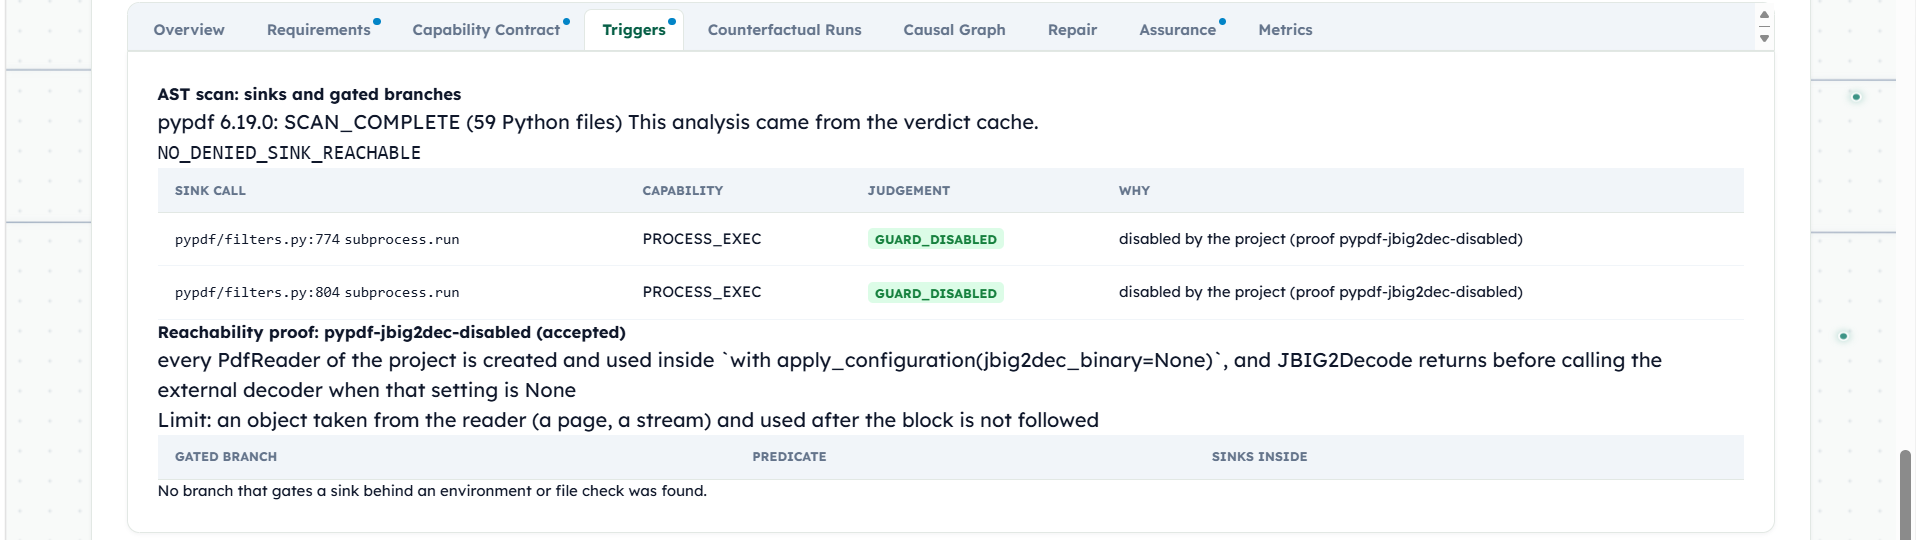
\includegraphics[width=0.9\linewidth]{figures/cavr/cavr-12-ast-scan-sinks.png}
    \caption[AST scan and sink judgement for pypdf 6.19.0]{Triggers tab for \texttt{pypdf} 6.19.0: the AST scan of 59 Python files, the two \texttt{subprocess.run} sinks judged \texttt{GUARD\_DISABLED}, and the accepted reachability proof with its stated limit.}
    \label{fig:cavr-ast-scan}
\end{figure}

\begin{sloppypar}
\textbf{Verdict cache.} \path{cache_key} refuses to build a key unless all eight fields are usable, then hashes their canonical JSON. \path{store} accepts only \texttt{VERIFIED} and \texttt{REJECTED} results. \path{lookup} uses a row only if its integrity digest matches and its own eight columns give the key it is filed under. Only the scan and sink analysis is cached. The download, the tree, the contract and the OSV query run on every request, because the first three are fields of the key and advisories change while the file does not.
\end{sloppypar}

\begin{sloppypar}
\textbf{Pip wrapper.} \path{main} removes the wrapper's own options, calls \path{verify_request} on the remaining pip command, prints the verdict and evidence, and returns the exit code. With \path{--install} and a \texttt{VERIFIED} verdict, \path{install_plan} writes one line \path{name==version} \path{--hash=sha256:<digest>} per node of the verified tree, and pip is run once with a fixed option list: \path{--isolated}, \path{--index-url} \path{https://pypi.org/simple/}, \path{--require-hashes}, \path{--no-deps} and \path{--only-binary} \path{:all:}. The user's own pip arguments are never passed to pip.
\end{sloppypar}

\begin{sloppypar}
\textbf{Dashboard.} \path{run_verification} runs the pipeline in a worker thread and publishes one event per stage that ran, with every value copied from the verdict. \path{stage_summary} builds the six-stage timeline (capture, gate, artifact, cache, analysis, verdict); a stage with no value is marked as not run. Two demo conditions exist and only replace the network transport: \texttt{tampered\_wheel} flips one bit of the downloaded file and \texttt{network\_off} fails every request. A run under a demo condition gets no store, so it is not logged, not cached and not counted in the metrics, and it downloads into its own directory.
\end{sloppypar}

\begin{sloppypar}
Figure~\ref{fig:cavr-timeline-verified} shows the page after chip 1: the six stages of \path{stage_summary} with the value each one returned, and the reasoning panel below them. A tick marks a stage that ran, not a stage that passed; the verdict is the status under the last stage. Figure~\ref{fig:cavr-verdict-verified} shows the verdict card for the same chip. The card prints two words: a header, which is \texttt{ALLOW} for \texttt{VERIFIED}, \texttt{BLOCK} for \texttt{REJECTED} and \texttt{BLOCK}, and \texttt{NEEDS\_REVIEW} for \texttt{UNRESOLVED}, and below it the policy state, which is the CAVR verdict. The screenshots in this report were taken in one browser session on 2026-10-11. The server had already verified pypdf 6.19.0 in that session, so this run shows a cache \texttt{HIT}.
\end{sloppypar}

\begin{figure}[htbp]
    \centering
    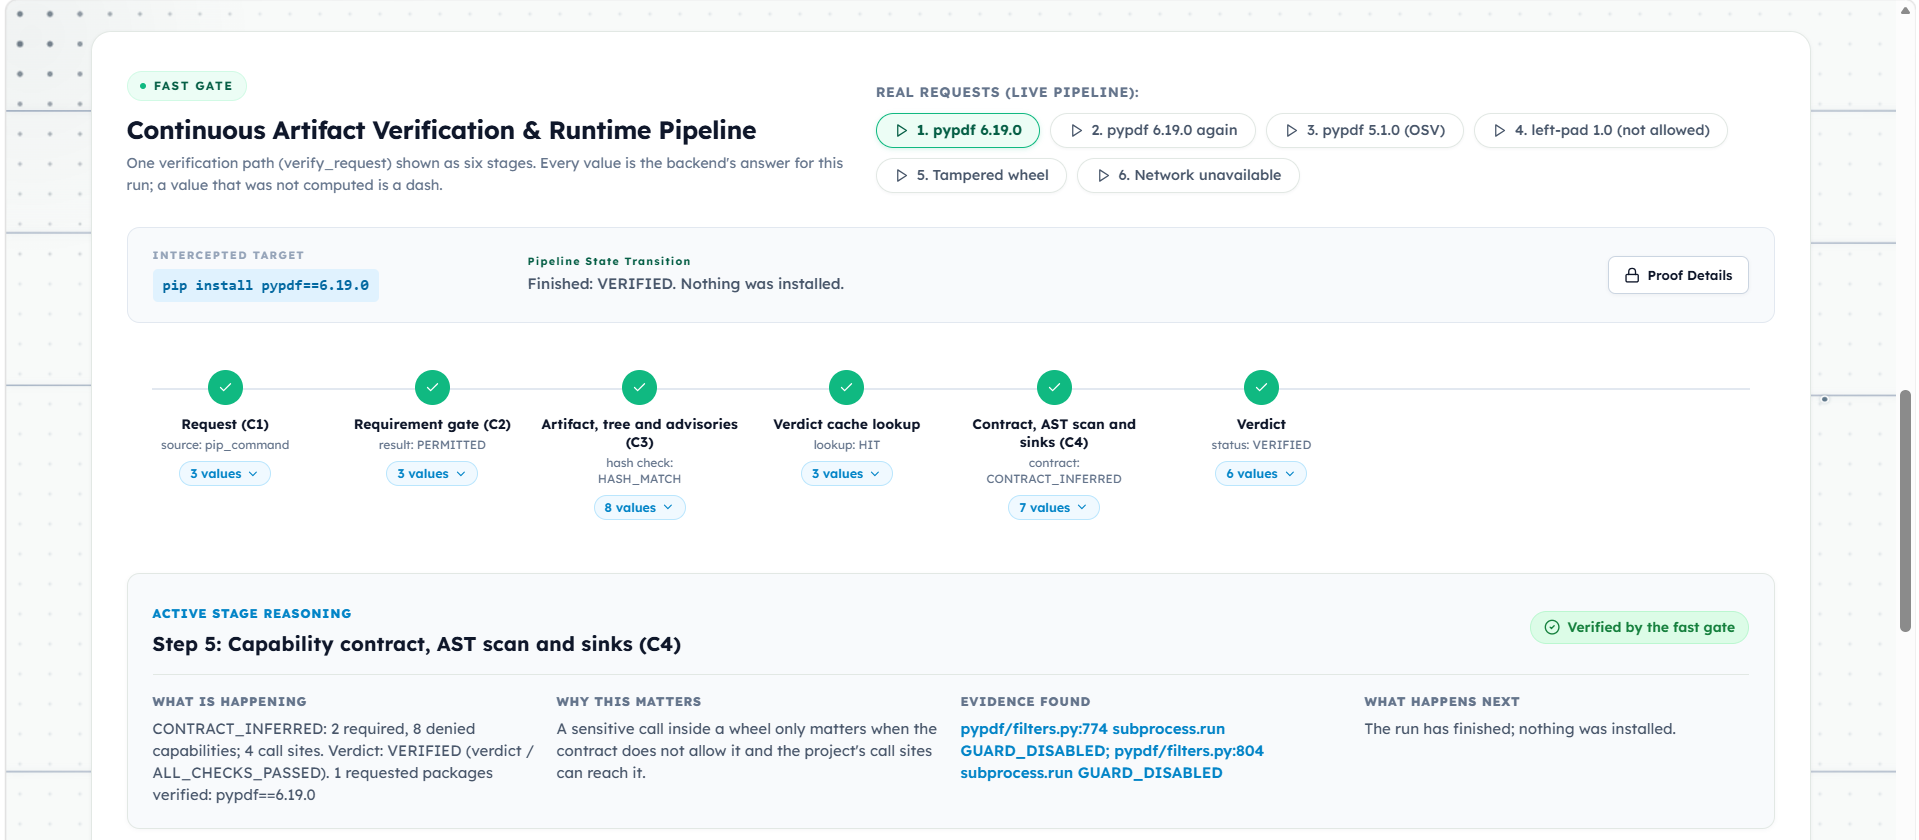
\includegraphics[width=0.9\linewidth]{figures/cavr/cavr-01-verified-pipeline.png}
    \caption[Six-stage timeline for a VERIFIED request]{CAVR page after chip 1, \texttt{pip install pypdf==6.19.0}: all six stages of the timeline ran and the verdict is \texttt{VERIFIED}. The cache lookup is a \texttt{HIT} because the server had verified this wheel earlier in the session. Nothing was installed.}
    \label{fig:cavr-timeline-verified}
\end{figure}

\begin{figure}[htbp]
    \centering
    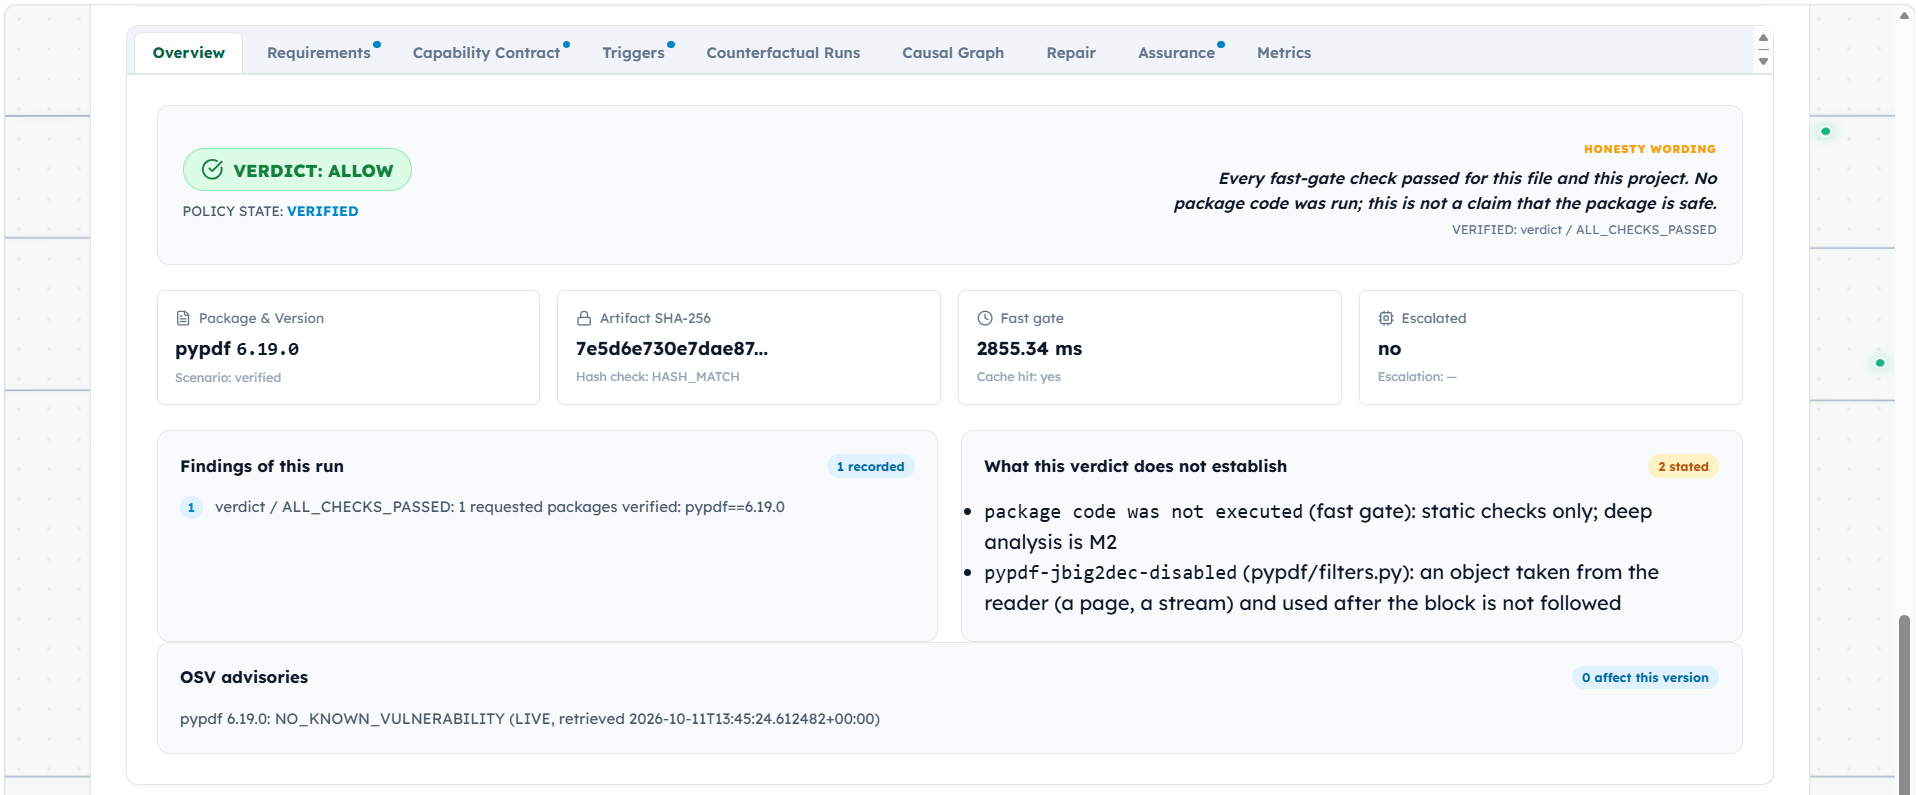
\includegraphics[width=0.9\linewidth]{figures/cavr/cavr-02-verified-verdict.png}
    \caption[Verdict card for a VERIFIED request]{Verdict card for \texttt{pypdf} 6.19.0: policy state \texttt{VERIFIED}, the artifact SHA-256 with \texttt{HASH\_MATCH}, the live OSV answer with no advisory for this version, and the two limits the verdict states.}
    \label{fig:cavr-verdict-verified}
\end{figure}

\begin{sloppypar}
Figure~\ref{fig:cavr-certificate-verified} shows the Assurance tab for another \texttt{VERIFIED} run of the same request in that session. The seven records are the \path{EvidenceChain} of the run, each hashed together with the SHA-256 of the record before it. The certificate below them is built by \path{certificate_for_verdict}: it repeats the verdict and lists the artifact, subtree and contract digests and the result of each check, with sandbox execution as \texttt{NOT\_RUN (M2)}. Figure~\ref{fig:cavr-certificate-limits} shows the limits the page prints below a certificate.
\end{sloppypar}

\begin{figure}[htbp]
    \centering
    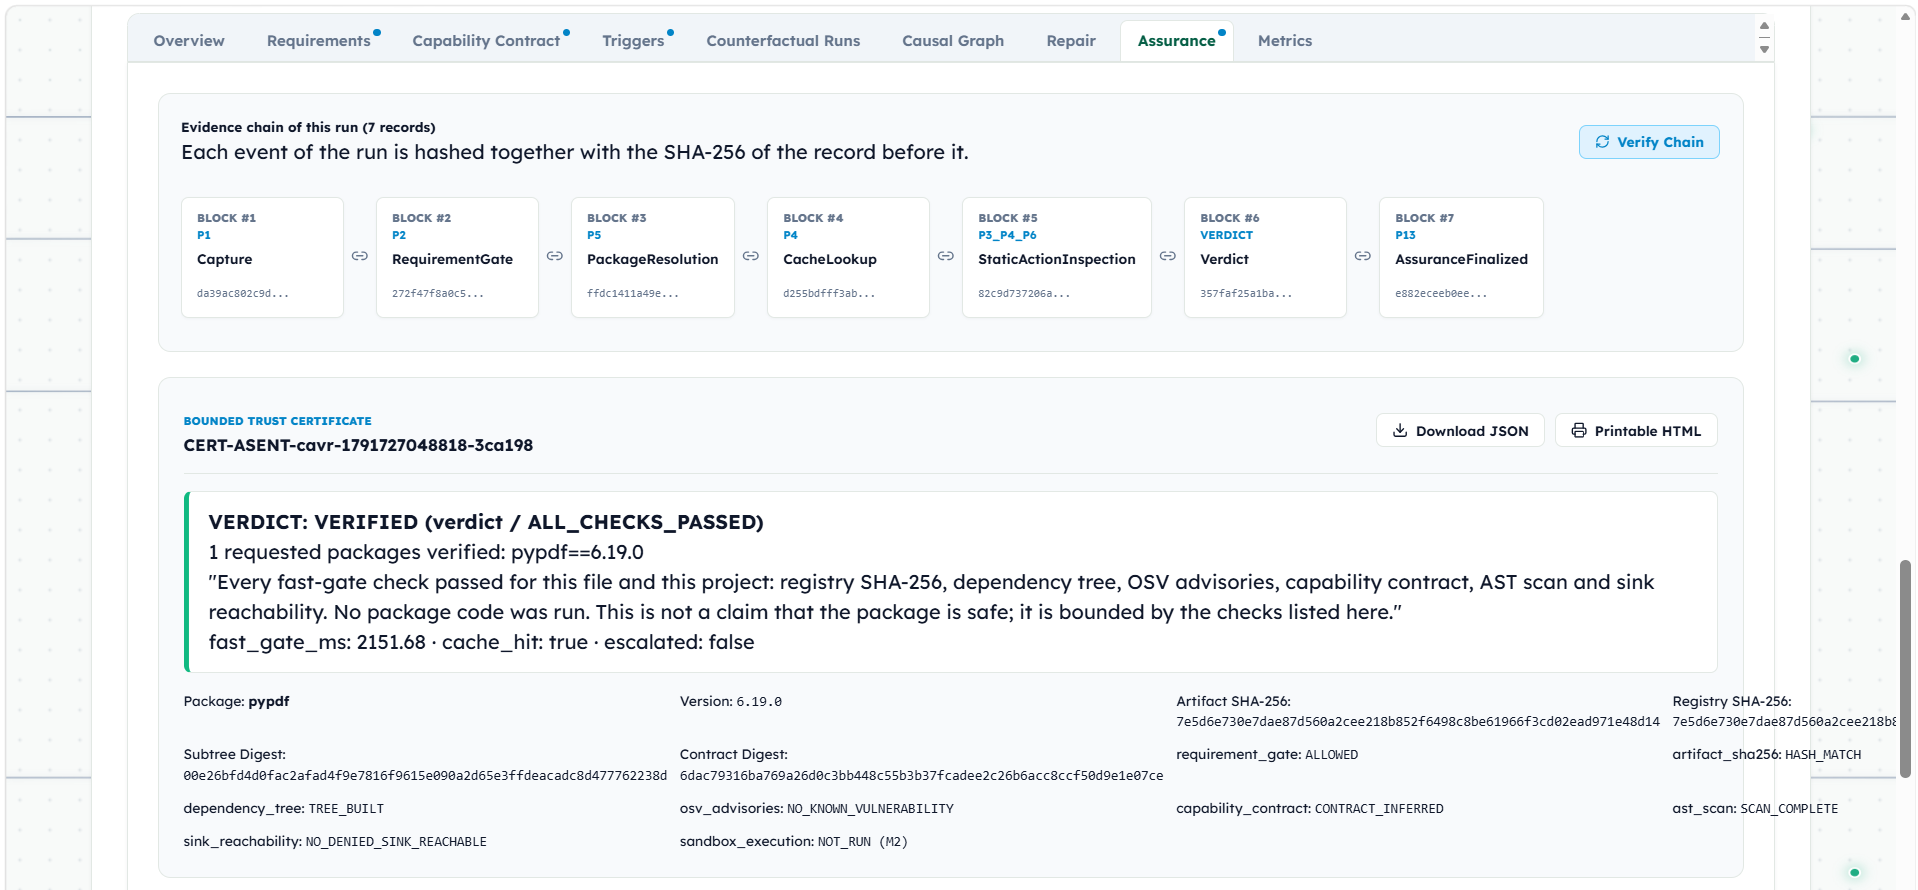
\includegraphics[width=0.9\linewidth]{figures/cavr/cavr-15-assurance-certificate-verified.png}
    \caption[Evidence chain and certificate for a VERIFIED run]{Assurance tab for a \texttt{VERIFIED} run of \texttt{pypdf} 6.19.0: the seven-record evidence chain and the bounded trust certificate with the digests and the result of each check. The right end of the registry digest is cut off by the browser window.}
    \label{fig:cavr-certificate-verified}
\end{figure}

\begin{figure}[htbp]
    \centering
    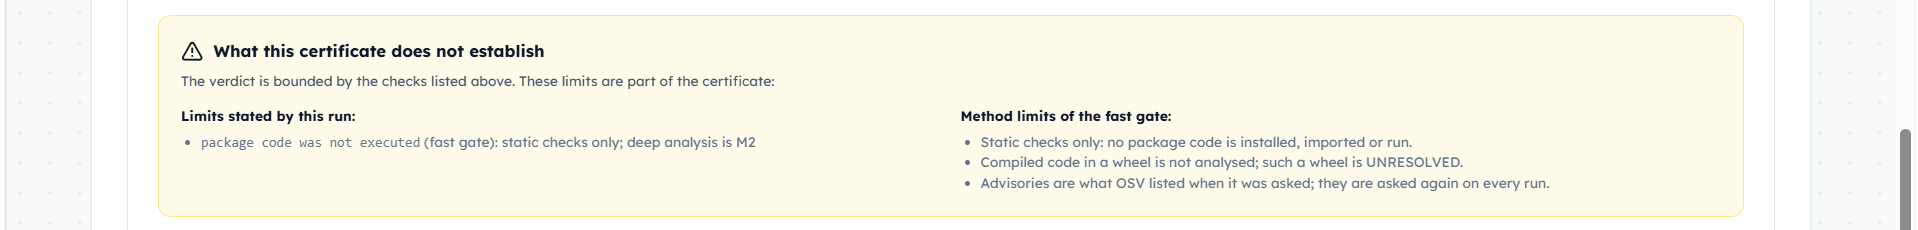
\includegraphics[width=0.9\linewidth]{figures/cavr/cavr-17-certificate-limits.png}
    \caption[Stated limits of a certificate]{``What this certificate does not establish'': the limits stated by the run and the method limits of the fast gate, as printed below a certificate.}
    \label{fig:cavr-certificate-limits}
\end{figure}

\subsection{Algorithms and Technical Decisions}
\setlength{\tabcolsep}{3pt}
\begin{longtable}{p{0.28\textwidth}p{0.25\textwidth}p{0.38\textwidth}}
\toprule
\textbf{Decision} & \textbf{Alternative considered} & \textbf{Why}\\
\midrule
\endhead
Unknown is \texttt{UNRESOLVED} at every stage. & Treat a missing value as zero or as clean. & A missing measurement is not a measurement of zero. A fail-open default would let a network error or an unread file end as \texttt{VERIFIED}.\\
Explicit pip option tables. & Skip every token that starts with a dash, as the old wrapper did. & The old way read the value of \path{-i}, \path{-t} or \path{--index-url} as a package name.\\
An unknown pip option makes the record incomplete. & Guess whether it takes a value, or ignore it. & Guessing either way could hide a package or invent one.\\
Hash the file after it is written, by reading it back. & Hash the chunks while streaming. & The evidence then describes the exact file the later stages open. The cost is reading the file twice.\\
Keep a mismatching file as \path{<filename>.rejected}. & Delete it, or keep the wheel name. & It stays as evidence, and no later stage can open it by its wheel name.\\
Verify the wheel for the running interpreter. & Verify every wheel of the release, or accept only pure-Python wheels. & It is the file pip would install on this machine. Pure-only would make every package with native wheels \texttt{UNRESOLVED}.\\
Check OSV ranges locally as a second reading of OSV's answer. & Trust OSV's answer alone. & If the two readings disagree, one of them is wrong, so the result is \texttt{UNRESOLVED} and not clean.\\
Cache only the scan and sink analysis; never the advisory result. & Cache the final verdict. & A cached \texttt{VERIFIED} must become \texttt{REJECTED} the day OSV lists the version, and a cached rejection must lift if the advisory is withdrawn.\\
Never store \texttt{UNRESOLVED} or \texttt{BLOCK} in the cache. & Cache everything with a short lifetime. & Storing \texttt{UNRESOLVED} would freeze a network failure. \texttt{BLOCK} is decided before any artifact exists, so there is nothing to key on.\\
Reachability is the import closure from the modules the project imports. & A full call graph, or treat every sink as reachable once the package is used. & It needs no execution and still leaves a real unreachable class, such as a command-line module nobody imports.\\
The wrapper passes pip a fixed option list and a generated hash-pinned file. & Append \path{--require-hashes} to the user's command. & An option the capture does not model could otherwise change what pip does.\\
No Docker gives \texttt{UNRESOLVED}; package code never runs on the host. & Keep the host run with the Python audit hook. & The audit hook is not isolation; untrusted code would run with the user's rights.\\
Demo runs get no store. & Log them under a separate label. & An arranged hash mismatch or a 3~ms network-off run is not a measurement, and without a store it cannot touch the cache.\\
Report \texttt{fast\_gate\_ms} per verdict and per cache lookup. & One p50 and p95 over all verdicts. & A \texttt{BLOCK} takes about 2~ms and would pull down the time reported for verifying a package.\\
\bottomrule
\end{longtable}
\setlength{\tabcolsep}{6pt}

\subsection{Tools, Frameworks and Technologies}
\begin{sloppypar}
CAVR is written in Python. The development machine runs Python 3.14.4 and the CI workflow runs Python 3.12. It uses the \texttt{packaging} library for requirement, version and wheel-tag parsing, \texttt{httpx} for HTTPS, and the standard-library modules \texttt{ast}, \texttt{zipfile}, \texttt{hashlib}, \texttt{shlex} and \texttt{sqlite3}. The endpoints are FastAPI routes. The page is React and TypeScript. Tests use pytest, and the page-rendering tests also need Node.js. The two external data sources are the PyPI JSON API with \path{files.pythonhosted.org} and the OSV database, reached through the existing \path{backend/integrations/osv_adapter.py}. GitHub Actions runs the suite with Docker and Podman disabled.
\end{sloppypar}

\begin{sloppypar}
Docker is needed only by the sandbox runner, which the fast gate does not call. Docker is not installed on the development machine, so the real container path has not been executed; every sandbox-runner test replaces the process launcher.
\end{sloppypar}

\begin{sloppypar}
\textbf{Tool use.} I used Claude Code (Anthropic) throughout this iteration. It generated the code changes in \path{backend/cavr/}, the tests in \path{tests/test_cavr_*.py}, the page components and the working notes, following a written plan and the branch rules in \path{CLAUDE.md}. Each batch of plan steps was then read by \texttt{cavr-reviewer}, a read-only Claude Code subagent, and the blocking findings were fixed in a separate commit. My part was to set the scope and the rules, approve the plan steps and the batch workflow, and make the decisions the notes record as mine: for the first step I read the four reviewer reports and decided the outcome of each finding, including which to defer; I chose between the options for the forged-report fix; I wrote the list of six demo issues and the expected verdict of each chip; and I reported the two CI failures and set the rule for fixing the second. For the batches in between, the notes record that the steps ran without a stop and list the open choices left for me. Verification was by pytest, by running new tests against the old code, by fault injection, and by live runs against PyPI and OSV. No project source code is sent to PyPI or OSV; they receive the package name and version only. \textbf{TODO: state which CAVR files I have since read line by line, and which open choices from the notes I have decided.}
\end{sloppypar}

\subsection{Reproducible Setup and Run Instructions}
On Linux, from the repository root:
\begin{sloppypar}
\begin{enumerate}
    \item \texttt{bash} \path{scripts/setup.sh} creates \path{.venv}, installs \path{requirements.lock.txt} and builds the dashboard. It needs Python 3.11 or newer, and npm to build the dashboard.
    \item \texttt{npm} \path{--prefix} \texttt{frontend} \texttt{run} \texttt{build} rebuilds the dashboard after any frontend change. The build output \path{frontend/dist} is not in Git.
    \item \texttt{export} \path{ASENT_DATA=$PWD/runtime-demo} selects an empty data directory, so the first request is a cache miss.
    \item \path{.venv/bin/python} \path{-m} \path{uvicorn} \path{backend.main:app} \path{--host} \path{127.0.0.1} \path{--port} \path{8000} starts the app with the same \texttt{ASENT\_DATA}. Open \path{http://127.0.0.1:8000} and go to the CAVR module.
    \item The pip wrapper is run as \path{.venv/bin/python} \path{-m} \path{backend.cavr.pip_shim} \path{--cavr-project} \path{backend/cavr/sample_project} \path{--cavr-policy} \path{backend/cavr/project_policy.json} \texttt{install} \path{pypdf==6.19.0}.
\end{enumerate}
\end{sloppypar}
The fast gate needs internet access to reach PyPI and OSV. Nothing is installed by any of these commands. The full demo script with the recorded output of every command is \path{docs/cavr-demo.md} on the \texttt{cavr} branch.

\subsection{Demonstration Evidence}\label{sec:cavr-demo}
\begin{sloppypar}
The six cases below are the six chips of the CAVR page. Each was run through \texttt{POST} \path{/api/cavr/run?scenario=<id>}, which is what a chip click calls. The output was recorded on 2026-10-11 at commit \texttt{42e2524} with Python 3.14.4 and Node.js v22.22.1 on WSL2, with internet access. Nothing in these runs uses fixture data. The time column is \texttt{fast\_gate\_ms}, the wall time of the whole request.
\end{sloppypar}

\setlength{\tabcolsep}{3pt}
\begin{longtable}{p{0.04\textwidth}p{0.24\textwidth}p{0.36\textwidth}p{0.11\textwidth}p{0.14\textwidth}}
\toprule
\textbf{No.} & \textbf{Request} & \textbf{Verdict, stage and rule} & \textbf{Cache} & \textbf{Time (ms)}\\
\midrule
\endhead
1 & \texttt{pip install pypdf==6.19.0} & \texttt{VERIFIED}, \texttt{verdict}, \texttt{ALL\_CHECKS\_PASSED}; \texttt{HASH\_MATCH} & \texttt{MISS} & 3912.65\\
2 & The same request again & \texttt{VERIFIED}, \texttt{verdict}, \texttt{ALL\_CHECKS\_PASSED}; \texttt{HASH\_MATCH} & \texttt{HIT} & 2117.81\\
3 & \texttt{pip install pypdf==5.1.0} & \texttt{REJECTED}, \texttt{advisories}, \texttt{KNOWN\_VULNERABILITY}; \texttt{HASH\_MATCH}; 97 advisories & \texttt{MISS} & 2919.3\\
4 & \texttt{pip install left-pad==1.0} & \texttt{BLOCK}, \texttt{gate}, \texttt{NOT\_ON\_ALLOWLIST}; nothing downloaded & not reached & 2.17\\
5 & \texttt{pip install pypdf==6.19.0}, one bit of the wheel flipped on the way in & \texttt{REJECTED}, \texttt{artifact}, \texttt{HASH\_MISMATCH} & not reached & 1582.34\\
6 & \texttt{pip install pypdf==6.19.0}, PyPI unreachable & \texttt{UNRESOLVED}, \texttt{artifact}, \texttt{REGISTRY\_UNAVAILABLE} & not reached & 3.09\\
\bottomrule
\end{longtable}
\setlength{\tabcolsep}{6pt}

\begin{sloppypar}
In cases 1 and 2 the SHA-256 computed from the downloaded file and the registry digest are both \path{7e5d6e730e7dae87d560a2cee218b852f6498c8be61966f3cd02ead971e48d14}. In case 5 the registry digest is the same value and the file that arrived hashes to \path{a52a19f9f614cd13e3f7544c78e5a44fc0996507c8b1b620abd45da5d73ee7b9}. The rejected file is kept under \path{quarantine-demo/tampered_wheel/}, and the genuine wheel in \path{quarantine/} had the same SHA-256 before and after the tampered run. In case 3 the reason names the count and the first three OSV identifiers (\texttt{GHSA-23w6-3w8w-8484}, \texttt{GHSA-248m-82v9-q6g6}, \texttt{GHSA-2q4j-m29v-hq73}) ``and 94 more''; the count grows when OSV publishes more. In case 4 the quarantine directory holds only the two pypdf wheels of cases 1 to 3. In case 6 the same request that was verified and cached in cases 1 and 2 is not served from the cache, because the SHA-256 of the downloaded file is one of the eight key fields.
\end{sloppypar}

\begin{sloppypar}
The blocks below are the recorded output of those runs, copied from \path{docs/cavr-demo.md}. Each was printed by the two helper functions of the demo script, which call \texttt{POST} \path{/api/cavr/run?scenario=<id>} and then read \texttt{GET} \path{/api/cavr/proof/{run_id}}. Lines longer than the page are wrapped here with an indent; nothing else is changed. The run id and \texttt{fast\_gate\_ms} differ on every run.
\end{sloppypar}

\noindent Case 1, chip ``1. pypdf 6.19.0'': verified, cache miss.
\begin{singlespace}
\scriptsize
\begin{verbatim}
run id: cavr-1791668207427-c7286f
request: pip install pypdf==6.19.0
verdict: VERIFIED | stage: verdict | rule: ALL_CHECKS_PASSED
reason: 1 requested packages verified: pypdf==6.19.0
demo condition: None
hash expected (registry): 7e5d6e730e7dae87d560a2cee218b852f6498c8be61966f3cd02ead971e48d14
hash of what arrived:     7e5d6e730e7dae87d560a2cee218b852f6498c8be61966f3cd02ead971e48d14
hash result: HASH_MATCH | matches: True
fast_gate_ms: 3912.65 | cache_hit: False | escalated: False | logged: True
  stage capture  ran         | source: pip_command
  stage gate     ran         | result: PERMITTED
  stage artifact ran         | hash check: HASH_MATCH
  stage cache    ran         | lookup: MISS
  stage analysis ran         | contract: CONTRACT_INFERRED
  stage verdict  ran         | status: VERIFIED
\end{verbatim}
\end{singlespace}

\noindent Case 3, chip ``3. pypdf 5.1.0 (OSV)'': the genuine wheel, rejected by the advisory check.
\begin{singlespace}
\scriptsize
\begin{verbatim}
run id: cavr-1791668213619-9f0f52
request: pip install pypdf==5.1.0
verdict: REJECTED | stage: advisories | rule: KNOWN_VULNERABILITY
reason: pypdf==5.1.0: pypdf 5.1.0 is affected by 97 known advisories: GHSA-23w6-3w8w-8484,
      GHSA-248m-82v9-q6g6, GHSA-2q4j-m29v-hq73 and 94 more
demo condition: None
hash expected (registry): 3bd4f503f4ebc58bae40d81e81a9176c400cbbac2ba2d877367595fb524dfdfc
hash of what arrived:     3bd4f503f4ebc58bae40d81e81a9176c400cbbac2ba2d877367595fb524dfdfc
hash result: HASH_MATCH | matches: True
fast_gate_ms: 2919.3 | cache_hit: False | escalated: False | logged: True
  stage capture  ran         | source: pip_command
  stage gate     ran         | result: PERMITTED
  stage artifact ran         | hash check: HASH_MATCH
  stage cache    ran         | lookup: MISS
  stage analysis ran         | contract: CONTRACT_INFERRED
  stage verdict  ran         | status: REJECTED
\end{verbatim}
\end{singlespace}

\noindent Case 4, chip ``4. left-pad 1.0 (not allowed)'': blocked at the gate. The last two lines are the listing of the quarantine directory, which holds only the wheels of cases 1 to 3.
\begin{singlespace}
\scriptsize
\begin{verbatim}
run id: cavr-1791668216623-a934f6
request: pip install left-pad==1.0
verdict: BLOCK | stage: gate | rule: NOT_ON_ALLOWLIST
reason: left-pad is not on the project allowlist
demo condition: None
hash expected (registry): None
hash of what arrived:     None
hash result: None | matches: None
fast_gate_ms: 2.17 | cache_hit: False | escalated: False | logged: True
  stage capture  ran         | source: pip_command
  stage gate     ran         | result: BLOCK
  stage artifact did not run | hash check: None
  stage cache    did not run | lookup: None
  stage analysis did not run | contract: None
  stage verdict  ran         | status: BLOCK
pypdf-5.1.0-py3-none-any.whl
pypdf-6.19.0-py3-none-any.whl
\end{verbatim}
\end{singlespace}

\noindent Case 5, chip ``5. Tampered wheel'': the first line is \texttt{sha256sum} of the genuine wheel before the run; the last four lines are the quarantine listing and \texttt{sha256sum} of the genuine wheel and of the rejected file after it.
\begin{singlespace}
\scriptsize
\begin{verbatim}
7e5d6e730e7dae87d560a2cee218b852f6498c8be61966f3cd02ead971e48d14
      runtime-demo/cavr/quarantine/pypdf-6.19.0-py3-none-any.whl
run id: cavr-1791668228892-f6e43c
request: pip install pypdf==6.19.0
verdict: REJECTED | stage: artifact | rule: HASH_MISMATCH
reason: pypdf==6.19.0: pypdf-6.19.0-py3-none-any.whl: SHA-256 of the downloaded file is
      a52a19f9f614cd13e3f7544c78e5a44fc0996507c8b1b620abd45da5d73ee7b9, the registry says
      7e5d6e730e7dae87d560a2cee218b852f6498c8be61966f3cd02ead971e48d14
demo condition: tampered_wheel
hash expected (registry): 7e5d6e730e7dae87d560a2cee218b852f6498c8be61966f3cd02ead971e48d14
hash of what arrived:     a52a19f9f614cd13e3f7544c78e5a44fc0996507c8b1b620abd45da5d73ee7b9
hash result: HASH_MISMATCH | matches: False
fast_gate_ms: 1582.34 | cache_hit: False | escalated: False | logged: False
  stage capture  ran         | source: pip_command
  stage gate     ran         | result: PERMITTED
  stage artifact ran         | hash check: HASH_MISMATCH
  stage cache    did not run | lookup: None
  stage analysis did not run | contract: None
  stage verdict  ran         | status: REJECTED
pypdf-5.1.0-py3-none-any.whl
pypdf-6.19.0-py3-none-any.whl
7e5d6e730e7dae87d560a2cee218b852f6498c8be61966f3cd02ead971e48d14
      runtime-demo/cavr/quarantine/pypdf-6.19.0-py3-none-any.whl
a52a19f9f614cd13e3f7544c78e5a44fc0996507c8b1b620abd45da5d73ee7b9
      runtime-demo/cavr/quarantine-demo/tampered_wheel/pypdf-6.19.0-py3-none-any.whl.rejected
\end{verbatim}
\end{singlespace}

\noindent Case 6, chip ``6. Network unavailable'': unresolved, although the same request was verified and cached in cases 1 and 2.
\begin{singlespace}
\scriptsize
\begin{verbatim}
run id: cavr-1791668230579-72878e
request: pip install pypdf==6.19.0
verdict: UNRESOLVED | stage: artifact | rule: REGISTRY_UNAVAILABLE
reason: pypdf==6.19.0: cannot read the registry: ConnectError: the network is off (dashboard demo
      condition)
demo condition: network_off
hash expected (registry): None
hash of what arrived:     None
hash result: REGISTRY_UNAVAILABLE | matches: None
fast_gate_ms: 3.09 | cache_hit: False | escalated: False | logged: False
  stage capture  ran         | source: pip_command
  stage gate     ran         | result: PERMITTED
  stage artifact ran         | hash check: REGISTRY_UNAVAILABLE
  stage cache    did not run | lookup: None
  stage analysis did not run | contract: None
  stage verdict  ran         | status: UNRESOLVED
\end{verbatim}
\end{singlespace}

The same requests were run through the pip wrapper in the same data directory:

\setlength{\tabcolsep}{3pt}
\begin{longtable}{p{0.40\textwidth}p{0.38\textwidth}p{0.12\textwidth}}
\toprule
\textbf{Wrapper request} & \textbf{Verdict, stage and rule} & \textbf{Exit code}\\
\midrule
\endhead
\texttt{install pypdf==6.19.0} & \texttt{VERIFIED}, \texttt{verdict}, \texttt{ALL\_CHECKS\_PASSED}; cache \texttt{HIT} & 0\\
\texttt{install pypdf==5.1.0} & \texttt{REJECTED}, \texttt{advisories}, \texttt{KNOWN\_VULNERABILITY} & 1\\
\texttt{install left-pad==1.0} & \texttt{BLOCK}, \texttt{gate}, \texttt{NOT\_ON\_ALLOWLIST} & 3\\
\texttt{install pypdf==6.19.0} with every HTTPS request sent to a local port where nothing listens & \texttt{UNRESOLVED}, \texttt{artifact}, \texttt{REGISTRY\_UNAVAILABLE} (``Connection refused'') & 2\\
\bottomrule
\end{longtable}
\setlength{\tabcolsep}{6pt}

\noindent Wrapper run for \texttt{pypdf==6.19.0}, with the evidence of every stage and exit code 0. It was run after cases 1 to 6 in the same data directory, so it is a cache hit on the analysis the dashboard stored.
\begin{singlespace}
\scriptsize
\begin{verbatim}
CAVR verdict: VERIFIED
  stage: verdict   rule: ALL_CHECKS_PASSED
  reason: 1 requested packages verified: pypdf==6.19.0
  request: pip install pypdf==6.19.0
  fast_gate_ms: 2161.04   cache_hit: True   escalated: False
  gate: PERMITTED (ALLOWED)   policy version:
      e4b357a45bb7400290f240991bbe174606fafa750e9fd08dba7fb18c0984fc46
package pypdf==6.19.0: VERIFIED (verdict / ALL_CHECKS_PASSED)
  reason: hash, tree, advisories and contract checked; 2 sink calls found; none is both denied by
      the contract and reachable from the project
  artifact: pypdf-6.19.0-py3-none-any.whl HASH_MATCH
    sha256 7e5d6e730e7dae87d560a2cee218b852f6498c8be61966f3cd02ead971e48d14
    registry 7e5d6e730e7dae87d560a2cee218b852f6498c8be61966f3cd02ead971e48d14
  tree: TREE_BUILT, 1 file(s), subtree digest
      00e26bfd4d0fac2afad4f9e7816f9615e090a2d65e3ffdeacadc8d477762238d
    pypdf==6.19.0 sha256 7e5d6e730e7dae87d560a2cee218b852f6498c8be61966f3cd02ead971e48d14
  contract: CONTRACT_INFERRED, 4 call site(s), digest
      6dac79316ba769a26d0c3bb448c55b3b37fcadee2c26b6acc8ccf50d9e1e07ce
  advisories: pypdf 6.19.0 NO_KNOWN_VULNERABILITY
  scan: pypdf SCAN_COMPLETE (59 Python files)
  sink: pypdf/filters.py:774 subprocess.run GUARD_DISABLED
  sink: pypdf/filters.py:804 subprocess.run GUARD_DISABLED
  cache: HIT
install: not requested; nothing was installed (run again with --install after a VERIFIED verdict)
exit code: 0
\end{verbatim}
\end{singlespace}

\begin{sloppypar}
The last wrapper run is a real connection failure with no demo switch. For the verified request the wrapper also printed the evidence of each stage: the tree has one node, the contract has four call sites, the scan read 59 Python files, and the two \texttt{subprocess.run} sinks in \path{pypdf/filters.py} were both judged \texttt{GUARD\_DISABLED}.
\end{sloppypar}

\begin{sloppypar}
\textbf{Metrics.} After cases 1 to 6 and one more click of chip 2, \texttt{GET} \path{/api/cavr/metrics} reported five logged verdicts: three \texttt{VERIFIED}, one \texttt{REJECTED} and one \texttt{BLOCK}. Cases 5 and 6 are demo-condition runs and are not logged. Two of the five verdicts were cache hits (0.4), which is two of the four verdicts that reached the cache lookup (0.5). The three \texttt{VERIFIED} requests took 3912.65~ms (miss), 2117.81~ms (hit) and 4524.49~ms (hit). A cache hit skips only the AST scan and the sink judgement; the wheel is still downloaded and OSV is still asked, so most of the time is network and one hit was slower than the miss. With one to three requests per group these are observations, not statistics, and I do not claim a speed-up from the cache.
\end{sloppypar}

\begin{sloppypar}
\textbf{Repository.} The \texttt{cavr} branch has 42 commits that are not on \texttt{origin/master}, dated 2026-10-09 to 2026-10-11, all under my name: 13 \texttt{feat(cavr)}, 12 \texttt{fix(cavr)}, one \texttt{refactor(cavr)}, one \texttt{test(cavr)}, 9 \texttt{docs(cavr)}, 4 \texttt{chore(cavr)} and two outside the module. Each plan step is one commit, and each review round has its own fix commit. The commits that carry the features of this chapter are:
\end{sloppypar}

\setlength{\tabcolsep}{3pt}
\begin{longtable}{p{0.13\textwidth}p{0.78\textwidth}}
\toprule
\textbf{Commit} & \textbf{What it contains}\\
\midrule
\endhead
\texttt{3be14db} & Refuse host execution of unpinned package source (sandbox runner).\\
\texttt{73f7892} & C1: parse \texttt{pip install} commands into capture records.\\
\texttt{4c053b6} & C1: capture \path{requirements.txt} edits.\\
\texttt{c018f30} & C2: fail-closed requirement gate.\\
\texttt{31dd229} & Review fix: close two fail-open paths in the gate.\\
\texttt{00b9332} & C3: fetch PyPI release metadata and verify the artifact SHA-256.\\
\texttt{3ba4970} & C3: read wheel metadata safely.\\
\texttt{3cb1a35} & C3: transitive tree and subtree digest.\\
\texttt{b7c98cf} & C3: OSV check with real version ranges.\\
\texttt{c72b56a} & C3: light AST risk scan of wheel sources.\\
\texttt{c9b8852} & Review fix: read \texttt{.pth} files the way \path{site.py} does.\\
\texttt{a188cb6} & C4: capability contract from real imports and call sites.\\
\texttt{d8e6367} & Eight-field verdict cache.\\
\texttt{c5c0ef4} & Single \path{verify_request} pipeline.\\
\texttt{002a69c} & Review fix: close fail-open paths in the sink judgement and the pypdf proof.\\
\texttt{1e17034} & Pip wrapper runs the pipeline before pip.\\
\texttt{ca5a0e2} & Dashboard API uses the pipeline.\\
\texttt{fe9fd4f} & Review fix: keep demo runs out of the report numbers; drop the old trusted-package endpoints.\\
\texttt{384ec4f} & Dashboard chips are six real requests from the scenario API.\\
\texttt{42e2524} & Tampered-wheel demo run works on its own copy. The demo outputs above were recorded at this commit.\\
\texttt{8cafa8a} & Review fix: no ``nothing found'' without a scan, no advisory count without an OSV answer.\\
\texttt{fd276d7} & Find pypdf call sites reached through a vendored local artifact.\\
\texttt{d63183d} & Fix the two defects found by CI. Head of the branch.\\
\bottomrule
\end{longtable}
\setlength{\tabcolsep}{6pt}

\begin{sloppypar}
\textbf{CI.} The workflow \path{.github/workflows/ci.yml} was added in commit \texttt{1d0fe31}. It has six jobs on Python 3.12: lint (byte-compile and a Bandit scan), the CAVR tests (\path{tests/test_cavr_*.py}), the SABLE isolation test, the shared and threat-repository tests, the full suite, and the frontend build. Commits \texttt{1b55cca} and \texttt{4b32eb5} make the test jobs stop Docker and move the \texttt{docker} and \texttt{podman} binaries away before pytest starts, so the sandbox tests run in the no-container mode; a job with a real Docker sandbox is deferred. The runs on the \texttt{cavr} branch are:
\end{sloppypar}

\setlength{\tabcolsep}{3pt}
\begin{longtable}{p{0.16\textwidth}p{0.12\textwidth}p{0.62\textwidth}}
\toprule
\textbf{Run} & \textbf{Commit} & \textbf{Result}\\
\midrule
\endhead
\href{https://github.com/SheharyarAli-Dev/Working-POC/actions/runs/38092518268}{38092518268} & \texttt{7c2bd6b} & Failed in the CAVR tests job and the full-suite job. \textbf{TODO: record which tests failed; the log was not available when this chapter was written.}\\
\href{https://github.com/SheharyarAli-Dev/Working-POC/actions/runs/38135800645}{38135800645} & \texttt{fd276d7} & Failed. CAVR tests job: 1 failed, 1238 passed, 26 skipped. Full-suite job: 2 failed, 1302 passed, 26 skipped. The other four jobs passed.\\
\href{https://github.com/SheharyarAli-Dev/Working-POC/actions/runs/38137109059}{38137109059} & \texttt{d63183d} & All six jobs passed. CAVR tests job: 1254 passed, 26 skipped. Full-suite job: 1319 passed, 26 skipped.\\
\bottomrule
\end{longtable}
\setlength{\tabcolsep}{6pt}

\begin{sloppypar}
The 26 skips in CI are the seven live tests, which need \texttt{CAVR\_LIVE=1}, and the 19 page-rendering tests, which need the frontend's Node modules in the test job. The two failures of run 38135800645 are described in the next subsection.
\end{sloppypar}

\begin{sloppypar}
\textbf{Screenshots.} The recorded output above was produced through the API, without a browser. The page was opened in a browser afterwards, on 2026-10-11, and the six chips were clicked. Case 1 in that session is shown in Figures~\ref{fig:cavr-timeline-verified} and~\ref{fig:cavr-verdict-verified}, and cases 3 to 6 are shown in Section~\ref{sec:cavr-edge}. These are separate runs from the ones recorded above, so the run ids and \texttt{fast\_gate\_ms} differ, and case 1 appears there as a cache \texttt{HIT}.
\end{sloppypar}

\subsection{Defects Found by CI}\label{sec:cavr-ci-defects}
\begin{sloppypar}
Run 38135800645 failed two tests that pass on the development machine. The development machine runs Python 3.14.4 and has no strace, Docker or Podman. CI runs Python 3.12 with Docker and Podman disabled. I reproduced both failures locally with Python 3.12.15 in a virtual environment built from \path{requirements.lock.txt} and a strace 6.19 binary on the path, and fixed both in commit \texttt{d63183d}.
\end{sloppypar}

\begin{sloppypar}
\textbf{Defect 1: \texttt{PermissionError} on Python 3.12.} The failing test was \path{test_directory_that_cannot_be_listed_makes_the_context_unresolved} in \path{tests/test_cavr_contract.py}. It gives the context extractor a project that contains a directory of mode 0 and expects \texttt{UNRESOLVED} with rule \texttt{SOURCE\_NOT\_READ}. In CI it ended with \texttt{PermissionError: [Errno 13] Permission denied}. The cause was in \path{_python_files} in \path{backend/cavr/context_extractor.py}: to skip virtual environments it asked whether \path{pyvenv.cfg} is a file inside each directory, using \path{Path.is_file()}. On a directory that may not be searched, \path{Path.is_file()} raises \texttt{PermissionError} on Python 3.12 and returns false on Python 3.14. So on 3.12 the walk crashed, and on 3.14 the unreadable directory was quietly treated as ``not a virtual environment''. Neither is the fail-closed behaviour the module requires.
\end{sloppypar}

\begin{sloppypar}
The fix replaces the \texttt{pathlib} calls with two helpers, \path{_is_symlink} and \path{_is_virtualenv}, that call \path{os.lstat} and \path{os.stat} directly. ``Not found'' is false; any other \texttt{OSError} is raised to the caller. \path{_python_files} catches it, adds the directory to \texttt{not\_read} and does not enter it, and any \texttt{not\_read} entry makes the context \texttt{UNRESOLVED} \texttt{SOURCE\_NOT\_READ}. The same change fixed two things the old code got wrong on Python 3.14: a directory of mode 444 was not reported as one unreadable directory, and a project directory under a closed parent was called missing. I chose \path{os.stat} over wrapping the \texttt{pathlib} call in \texttt{try} because \texttt{pathlib} hides the error on 3.14, so only the direct call behaves the same on both versions. Four test functions with six cases were added to \path{tests/test_cavr_contract.py}, including \path{test_virtualenv_check_that_fails_makes_the_directory_not_read_on_every_python}, which produces the 3.12 behaviour on any Python by making \path{os.stat} refuse.
\end{sloppypar}

\begin{sloppypar}
\textbf{Defect 2: the no-container mode lost a network event.} The failing test was \path{test_controlled_dormant_execution} in \path{tests/test_modules.py}, with \texttt{assert False} on \texttt{causal\_confirmed}. The test runs the inert lab fixture twice, as a normal run and as the activated counterfactual run, and expects the canary marker to reach the local listener only in the activated run. Without a container the lab runner, \path{run_counterfactual} in \path{backend/cavr/sandbox.py}, uses strace as its monitor when strace is available (execution mode \texttt{PINNED\_INERT\_LAB\_STRACE}) and Python audit events otherwise (\texttt{PINNED\_INERT\_LAB\_PYTHON\_AUDIT}). The development machine has no strace, so it had only ever run the audit mode. The CI log does not print the execution mode; that the runner used strace is concluded from the local reproduction, where the test fails with strace on the path and passes without it, on Python 3.12 and 3.14 alike.
\end{sloppypar}

\begin{sloppypar}
The cause was in \path{normalize} in \path{backend/cavr/runtime_monitor.py}, which turns strace lines into events. It skipped every line whose result is \texttt{-1}. The lab file connects with \path{socket.create_connection} and a timeout, which is a non-blocking connect, and strace prints a non-blocking connect that has started as a \texttt{-1} result (the line is wrapped here):
\end{sloppypar}
\begin{singlespace}
\scriptsize
\begin{verbatim}
connect(4, {sa_family=AF_INET, sin_port=htons(18765), sin_addr=inet_addr("127.0.0.1")}, 16)
      = -1 EINPROGRESS
\end{verbatim}
\end{singlespace}
\begin{sloppypar}
\noindent That line was dropped, so the strace run had no \texttt{NETWORK\_CONNECT} event, no \texttt{NETWORK\_CONNECT} violation and no confirmed secret-read-then-connect correlation. The verdict was still \texttt{REJECTED} and the canary was still received in both modes; what was missing was one event and the evidence built on it. The fix keeps a \texttt{connect} line with \texttt{-1 EINPROGRESS}, because that result means the connection has started and not that it failed. Every other failed system call is still skipped: a refused connect made no connection, and counting attempts belongs to the later sandbox work. I did not weaken the test. Two assertions were added to it (a \texttt{NETWORK\_CONNECT} event in the activated run and none in the normal run), the execution mode is now printed in its assertion messages, and \path{tests/test_cavr_runtime_monitor.py} was added with five test functions and nine cases on eight recorded lines of the real trace. \path{test_the_connection_alone_is_not_a_confirmed_flow} checks that a connect without the received marker, with another payload, without the read, or before the read is not a confirmed flow.
\end{sloppypar}

\begin{sloppypar}
\textbf{After the fix.} The old code failed 9 of the new tests on Python 3.14 without strace and 13 on Python 3.12 with strace, the two CI failures among them. With the fix the full suite reported 1338 passed, 0 failed and 7 skipped on Python 3.14.4 without strace and the same on Python 3.12.15 with strace, and CI run 38137109059 on \texttt{d63183d} passed all six jobs. Three limits remain: a refused or blocked connect and a failed open of a secret file still leave no event; an \texttt{EINPROGRESS} connect is recorded without checking that it completed; and the Docker and Podman modes have not been run anywhere, because neither is installed on the development machine and CI disables both.
\end{sloppypar}

\subsection{Known Limitations}
\begin{itemize}
    \item The fast gate handles PyPI wheels only. A release with no wheel, and VCS, URL and local-path requirements, end \texttt{UNRESOLVED}. npm is not handled.
    \item No package is executed. Behaviour that only appears at run time, and native code, are outside the fast gate; a wheel with a native extension is \texttt{UNRESOLVED}.
    \item The shared orchestrator still calls the older analyzer in \path{backend/cavr/analyzer.py}, which does not go through \path{verify_request}. Moving it was stopped for a decision: the older analyzer accepts PyPI's advisory list when no OSV answer is stored, the pipeline does not, and the change would turn the orchestrator's safe scenario into \texttt{UNRESOLVED} offline.
    \item The advisory record the older analyzer relies on was retrieved on 2026-09-25 and is accepted for 30 days. From 2026-10-25 the integration tests that need pypdf \texttt{VERIFIED} on that path will fail unless a fresh advisory answer is stored.
    \item The \texttt{GUARD\_DISABLED} proof is written for pypdf only. Reachability is an import closure, not a call graph, and cannot see imports built at run time other than \path{__import__} and \path{importlib.import_module}.
    \item Every run downloads the tree again; the cache saves the scan, not the network.
    \item The cache integrity digest is a plain SHA-256. It detects damage and single-column edits. A keyed digest is deferred.
    \item The real Docker path of the sandbox runner has not been executed.
    \item The policy still approves \texttt{pdf-clean-extractor==1.0.0}, a name with no release on PyPI.
    \item The timeline fills in when the verdict is known, not stage by stage, and a tick means the stage ran, not that it passed.
\end{itemize}
